\documentclass{article}

% Language setting
% Replace `english' with e.g. `spanish' to change the document language
\usepackage[english]{babel}

% Set page size and margins
% Replace `letterpaper' with `a4paper' for UK/EU standard size
\usepackage[letterpaper,top=2cm,bottom=2cm,left=3cm,right=3cm,marginparwidth=1.75cm]{geometry}

% Useful packages
\usepackage{amsmath}
\usepackage{graphicx}
\usepackage{float} % u preambuli
\usepackage[colorlinks=true, allcolors=blue]{hyperref}
\usepackage{url}

% Bibliography management with BibTeX
\usepackage[numbers]{natbib}       % For citation styles
\bibliographystyle{unsrt}          % Citation style (you can use "unsrt", "alpha", etc.)

\title{Face Recognition System Using CLIP and FAISS for Scalable and Real-Time Identification}
\author{You}

\begin{document}
\maketitle

\begin{abstract}
% Mislin da za abstract ne tribaju reference
Face recognition is increasingly being adopted in industries such as education, security, and personalized services. This research introduces a face recognition system that leverages the embedding capabilities of the CLIP model. CLIP, a model trained on multimodal data, such as images and videos, generates high-dimensional features, which are then stored in a vector store for further queries. The system is designed to facilitate accurate real-time identification, with potential applications in areas such as attendance tracking and security screening. Specific use cases include event check-ins, implementation of advanced security systems, and more.
The process involves encoding known faces into high-dimensional vectors, indexing them using a vector store FAISS, and comparing them to unknown images based on cosine similarity. Experimental results demonstrate a high accuracy that exceeds 90\% and a performance efficiency even in datasets with a high volume of entries.
\end{abstract}

\subsection*{Introduction}
\hspace*{1.00cm}In today's digital age, facial recognition technologies play a key role in transforming how we interact with computer systems, secure spaces, and optimize everyday processes. Facial recognition is one of the fastest growing fields in biometric authentication, enabling fast and reliable identification of individuals without the need for physical contact or additional interaction\cite{article}. With the increasing availability of advanced computational resources and sophisticated algorithms, implementing facial recognition systems has become an indispensable tool across various industries.

\hspace*{1.00cm}The applications of this technology are diverse and span multiple sectors. In education, facial recognition can be used for automated student attendance tracking, allowing for more efficient monitoring and record-keeping. In the security sector, this technology enables the identification of suspicious individuals and enhances surveillance in public and private spaces, significantly contributing to crime prevention and increased safety. Additionally, in personalized services, facial recognition helps tailor user experiences by providing access to relevant information and services based on the user's identity\cite{parmar2014facerecognitionmethods}.


\hspace*{1.00cm}The goal of this research is to develop and evaluate an efficient facial recognition system that leverages the capabilities of the CLIP (Contrastive Language-Image Pre-Training) model to extract high-dimensional features from images and video recordings. This system, based on vector search techniques used in FAISS (Facebook AI Similarity Search), enables fast and accurate real-time facial identification. Through experimental evaluation, the research aims to demonstrate how the combination of advanced machine learning techniques and optimized search algorithms can enhance the accuracy and performance of existing facial recognition systems, with potential applications in security systems, attendance tracking, and other relevant fields.


\subsection*{Related Work}

\hspace*{1.00cm}FAISS (Facebook AI Similarity Search)\cite{faiss2025} and CLIP (Contrastive Language-Image Pretraining)\cite{luu2024clip} represent two advanced approaches in the fields of computer vision and natural language processing for data processing and retrieval. FAISS is a highly efficient system for vector similarity search, optimized to handle large databases. Its applications include image retrieval based on visual similarity, biometric facial recognition systems, recommendation systems, and semantic search for textual data and genetic sequences. It is particularly useful in IoT data analysis and anomaly detection, enabling fast comparisons of time series data and sensor patterns. Furthermore, FAISS is utilized in accelerated document search systems, user behavior analysis, and real-time data classification, significantly improving the scalability and efficiency of machine learning models.

\hspace*{1.00cm}On the other hand, CLIP is a transformer-based model trained on a large dataset combining images and descriptive texts, allowing it to understand visual content in the context of natural language. Its applications include image retrieval based on textual queries, automatic image captioning, zero-shot classification, and improving generative image models such as DALL·E and Stable Diffusion. CLIP is also used for content moderation, video analysis, autonomous system interactions with the environment, and in creative industries for generating artistic visuals based on semantic descriptions.

\hspace*{1.00cm}Although FAISS and CLIP have been applied individually in various domains, no implementation has been recorded that combines them for scalable real-time facial recognition. This work introduces the first such approach, leveraging CLIP’s capabilities to generate robust facial representations and FAISS’s efficiency for extremely fast searches within large databases. The integration of these two models enables the development of advanced multimodal data processing systems, providing more efficient search and classification methods across a wide range of applications, from security systems to creative industries. Our implementation not only enhances the speed and accuracy of facial identification, but also unlocks new possibilities in the field of computer vision that have not yet been explored.

\subsection*{Methodology and implementation}
\hspace*{1.00cm}The described system is implemented in Python using CLIP for embedding extraction from images and FAISS for fast search. Video recordings of human faces are processed into frames. The dataset consists of 50 classes, each class representing one individual, with two videos per class — one for "training" and the other for "validation."

\hspace*{1.00cm}For facial recognition, the system first loads known face images using the load\_known\_faces function, which iterates through directories labeled with class names (individuals). Each class contains a subdirectory named train, where images used for "learning" are stored. For each image in the training directory, the function add\_known\_face() is called, which extracts the image embedding using the CLIP model and associates it with the corresponding class. This process builds a database of known faces, that is later used for recognition.

\begin{figure}[H]
    \centering
    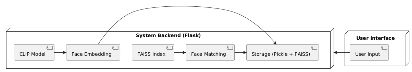
\includegraphics[width=0.8\linewidth]{converted_images/schema_overview.pdf}
      \textbf{Image 1:} Schema overview.
\end{figure}


\hspace*{1.00cm}After extracting embeddings, the computed vectors are organized into a FAISS index using the build\_index function. FAISS enables fast vector search in high-dimensional space using the L2 distance, also known as Euclidean distance.\cite{brownleeDistance}

The L2 distance between two vectors A = (a1, a2, ..., an) and B = (b1, b2, ..., bn) is defined as:

\begin{figure}[H]
    \centering
    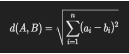
\includegraphics[width=0.20\linewidth]{converted_images/formula.pdf}
    \textbf{Image 2:} L2 distance.
\end{figure}

\hspace*{1.00cm}This metric measures the physical distance between two points in an n-dimensional space and is used to compare face embeddings (elements of each face) — the smaller the distance, the more similar embeddings. FAISS enables efficient nearest-neighbor search using this metric, speeding up the recognition process and avoiding linear search.

\hspace*{1.00cm}In our system, FAISS is used by storing all known face embeddings in an IndexFlatL2 index, which allows for fast search based on L2 distance. When adding a new embedding, it is simply inserted into the index along with its corresponding class label. When recognizing a new face, the embedding of the input image is compared with the embeddings in the FAISS index, and the system finds the k2 nearest neighbors (embeddings with the smallest L2 distance). These results are then used for classification through a voting method using the \texttt{classify\_face()} function among the first k1 results, the class that appears most frequently is selected by counting all occurrences of each class in that set. If the similarity threshold is not met, additional results (k1 to k2) are included to improve the decision.

The class with the most votes becomes the final prediction, unless no class meets the criteria, in which case the face is labeled as "Unknown".

\begin{figure}[H]
    \centering
    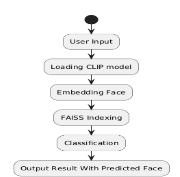
\includegraphics[width=0.6\linewidth]{converted_images/flowchart.pdf}
    \textbf{Image 3:} System flowchart.
\end{figure}

CLIP embedding example (face image for input and corresponding face embedding for output):
\begin{figure}[H]
    \centering
    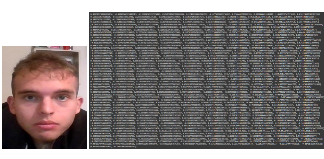
\includegraphics[width=0.6\linewidth]{converted_images/embeddings.pdf}
    \textbf{Image 4:} Embeddings example.
\end{figure}

\begin{figure}[H]
    \centering
    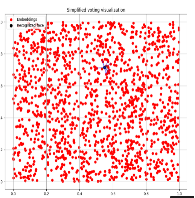
\includegraphics[width=0.6\linewidth]{converted_images/voting.pdf}
    \textbf{Image 5:} Simplified voting visualization.
\end{figure}

\subsection*{Experiments, tests and results}
\hspace*{1.00cm} First, the system was tested on a dataset of approximately 500 classes, where each person had 1 video, using some frames for training and the rest for validation (80-20 split). In this case, the results showed \texttt{100\%} accuracy because the training and validation data were nearly identical. Furthermore, to achieve more realistic results, the ytfaces\cite{ytfaces} dataset was used, which consists of videos of people in different environments. This approach was chosen because human faces in videos can successfully simulate the input the system would receive when using camera input for live recognition. From the dataset, 2 videos were extracted for each class to simulate facial scanning under different conditions during evaluation.

\begin{figure}[H]
    \centering
    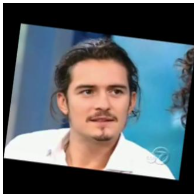
\includegraphics[width=0.4\linewidth]{converted_images/train_ex.pdf}
    \textbf{Image 6:} An example of train image.
\end{figure}
\begin{figure}[H]
    \centering
    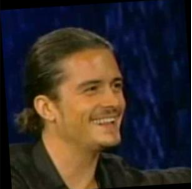
\includegraphics[width=0.4\linewidth]{converted_images/val_ex.pdf}
    \textbf{Image 7:} An example of val image.
\end{figure}

\subsubsection*{Evaluation process}
\hspace*{1.00cm}After defining the dataset, an extensive procedure was carried out to test various combinations of parameters k1, k2, and threshold. A grid search\cite{pedregosa2011scikit} was used for an efficient parameter search. The following parameter ranges were defined:
k1: 1-9
k2: 2-10
threshold: 0.5 - 1.0 with a step of 0.01
Additionally, a condition was defined to skip combinations where k1 and k2 are equal and where k2 is smaller than k1, in order to avoid meaningless steps in the search.
The testing and evaluation process was carried out by forwarding each image from all validation folders to CLIP to create its embeddings. Then, the embeddings were normalized for easier comparison using linalg.norm\cite{numpy_norm}.

\hspace*{1.00cm}For each embedding from the validation folder, a class prediction, i.e., face recognition, was performed. The true label and predicted label values were also saved for each image, which defines the actual class to which the image belongs and the class predicted by the model. If they are the same, it is a correct classification. If they differ, it indicates an error in prediction. The prediction is made by taking each validation embedding and comparing it with the known embeddings extracted from the training images, finding the most similar embedding (with the smallest distance). Once the system determines which class the most similar embeddings belong to, the validation embedding is assigned to that same class and recorded as a prediction, with an automatic accuracy check.

\hspace*{1.00cm}The minimum threshold was intentionally set to 0.5 because predictions with a lower threshold would be meaningless due to excessive strictness. The higher the threshold, the more images are considered, and the number of predictions increases. (Lower threshold... stricter decision and vice versa.)

\hspace*{1.00cm}During the evaluation of the results, the values obtained for each step of the search were automatically saved in the file \texttt{grid\_search\_results} . Specifically, it contains the following values: \texttt{k1, k2, threshold, precision, recall, f1, tp, fp, tn, fn}.\cite{powers2011evaluation}

\begin{figure}[H]
    \centering
    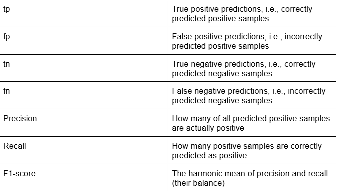
\includegraphics[width=0.8\linewidth]{converted_images/metrics.pdf}
    \textbf{Image 8:} Metrics overview.
\end{figure}


\hspace*{1.00cm}As the output of each step of the grid search, a row of data was generated with the k1, k2, and threshold parameters, along with the results produced by that combination of parameters. For example:
k1, k2, threshold, precision, recall, f1, tp, fp, tn, fn
 (1, 2, 1.0, 0.7305, 0.7305, 0.677, 2702, 991, 46577, 991)
Each individual parameter combination generated evaluation metrics that allowed for the analysis of the model's performance. The results were displayed in tabular form, including the used parameter values and the obtained metrics: precision, recall, F1-score, as well as the absolute values of true positives (TP), false positives (FP), true negatives (TN), and false negatives (FN). This output provides a detailed understanding of how changes in hyperparameters affect classification performance, enabling the selection of the optimal combination that achieves the best balance between the model's output metrics. 

% author work
\hspace*{1.00cm} For example, the configuration k1=1, k2=2, and threshold=1.0 resulted in precision=0.7305 and recall=0.7305, with the corresponding number of correct and incorrect classifications (TP=2702, FP=991, TN=46577, FN=991). By analyzing numerous results of this type, it is possible to assess the ideal balance between different metrics and adjust the model to achieve optimal classification efficiency in face recognition.

% author work
\hspace*{1.00cm}During the evaluation, the system's performance was monitored for different dataset sizes. As one might logically conclude, the metrics mainly decrease as the number of classes and images increases. Below 25 classes, the performance was perfect because the number of embeddings was small enough to prevent misclassifications due to the ample space in the embedding space.

\begin{figure}[H]
    \centering
    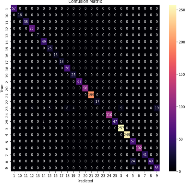
\includegraphics[width=0.70\linewidth]{converted_images/conf_mat1.pdf}
    \textbf{Image 9:} Confusion matrix with no misclassifications (25 classes).
\end{figure}

\subsubsection*{Effects of augmentation}

In the experimental phase, data augmentation\cite{yang2022image} for the training set was tested using techniques such as mirroring, rotation, cropping, blurring, etc. This approach significantly worsened the model's performance and deviated the evaluation method from the intended real-life use case. Namely, recognizing over-augmented images is quite difficult even with the naked eye, and it also has too much of an impact on the embeddings, making the distances too large for a valid match. Classic augmentation techniques (rotation, cropping, mirroring, blurring, etc.) were tested, but they were completely useless in real-life face recognition scenarios. In real-world situations, a person will not have a distorted or artificially modified face, as such augmentations are impossible in a real-life application of the system. The only real variations are changes in lighting and slight changes in the angle of the shot, which the system can still recognize. However, augmentations beyond that, such as rotation and contrast changes, lose their meaning. In the real world, more realistic "augmentations" include changes in hairstyle, growing a beard, makeup, etc., but these have little impact on the embeddings, as they don't significantly alter the key features of the face.

Example of train image and its valid matching validation image:
\begin{figure}[H]
    \centering
    
\includegraphics[width=0.8\linewidth]{converted_images/train_embd.pdf}
    \textbf{Image 10:} Train example.
\end{figure}
\begin{figure}[H]
    \centering
    
\includegraphics[width=0.8\linewidth]{converted_images/val_embd.pdf}
    \textbf{Image 11:} Val example.
\end{figure}

\begin{figure}[H]
    \centering
    
\includegraphics[width=0.8\linewidth]{converted_images/augment_embd.pdf}
    \textbf{Image 12:} Example of image with applied augmentation.
\end{figure}

\subsubsection*{Testing limitations}

% ovo je totalni author work
\hspace*{1.00cm}With 25 classes, there are minor misclassifications on certain similar images, but they are almost negligible, and each class is mostly correctly predicted overall. At 50 classes, the classification drops to \texttt{73\%}. A way to improve the results would definitely be to manually record 50 or more people in 2 videos under different conditions, which would provide higher quality test data and better embeddings. This part will be further explored during the scalability test evaluation.
Testing and validation were carried out by comparing predictions on the validation set with images from the training set, rather than real-time live input. Although this evaluation method is necessary, it does not fully reflect the challenges of real-time face recognition from a live feed, where factors such as lighting changes, different facial angles, facial expressions, and resolution variations can further impact model performance, but it also excludes some advantages that live testing provides. Unfortunately, due to limitations in standard experimental protocols, simulating these real-world conditions through the validation set currently represents the closest possible method of testing before implementation in real-time face recognition systems. Using a live feed allows for the analysis of many more consecutive frames in a shorter time, which enables the aggregation of predictions and reduces the impact of certain anomalies that may occur on individual images due to poor lighting, shooting angles, blurriness, etc. Instead of relying on static images, the system can collect more facial samples from the user over time, improving recognition reliability. This approach is particularly useful in dynamic systems where the goal is to achieve stable and precise recognition, such as security systems or contactless authentication.

\hspace*{1.00cm}Furthermore, live input enables adaptive techniques such as face tracking, where the model can continuously correct and improve detection by analyzing micro-movements and different facial expressions. This flexibility often leads to better overall accuracy in real-world environments than would be expected based on validation results obtained from traditional static image testing methods.

\subsubsection*{FAISS Implementation}
% ref na PCA članak
% opet na FAISS
\hspace*{1.00cm}Face embeddings were visualized in a two-dimensional space using Principal Component Analysis (PCA)\cite{lever2017pca}, which reduced the dimensionality by transforming multi-dimensional data into a smaller number of principal components, retaining as much variability as possible from the original data and their placement within the Clip embedding space. This approach provided insight into their distribution and mutual relationships. Some overlap between embeddings of different classes was observed, indicating challenges in distinguishing very similar faces. The overlap was especially pronounced for individuals with similar facial features, lighting, or expressions, making simple recognition methods more difficult. The more similar classes there are in the system and the larger the number of their instances, the greater the overlap, making it harder to clearly separate the classes, thus increasing the risk of misclassification, or confusion between classes that are close within the space. Two potential simple solutions would involve reducing the total number of classes or reducing the number of instances per class, but neither option is satisfactory. This situation highlights the need for advanced search methods, such as FAISS, which allows for fast and precise identification despite the overlap of embeddings.

\begin{figure}[H]
    \centering
    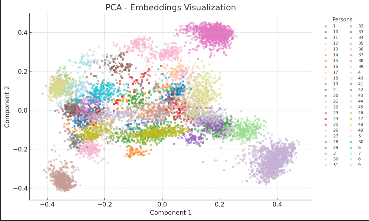
\includegraphics[width=0.5\linewidth]{converted_images/pca.pdf}
    \textbf{Image 13:} Realistic depiction of classes and their overlap
\end{figure}

% FAISS again
\hspace*{1.00cm}To address the problem of increasing overlap, FAISS (Facebook AI Similarity Search) was introduced, an optimized system for similarity search in large embedding spaces. FAISS uses efficient data structures such as ANN (Approximate Nearest Neighbors) search and quantization to speed up the recognition process and reduce the negative effects of overlap. This allows for more accurate and faster classification of instances, despite the increased data density in the space. The previously mentioned k1 and k2 parameters are specifically related to FAISS and represent how many matches it seeks in each step of embedding classification.

\begin{figure}[H]
    \centering
    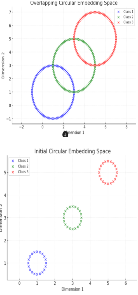
\includegraphics[width=0.50\linewidth]{converted_images/y_faiss.pdf}
    \textbf{Image 14:} Simplified depiction of overlap
\end{figure}

\subsubsection*{Reaching peak performance}
% autorski work
\hspace*{1.00cm}After a certain threshold value, the model reaches its maximum classification potential, where further increases in the threshold no longer affect the metrics. This indicates a high confidence in its decisions and the ability to clearly separate positive and negative examples. All positive classifications are above a certain confidence threshold, while negative ones are below it, meaning the model consistently and accurately makes decisions without uncertain predictions in the middle probability range. This effect confirms the robustness of the model and its resistance to threshold changes, achieving optimal accuracy in real-world scenarios. This is especially useful in systems where classification reliability is crucial, and further adjustment can only be used for fine-tuning the model in specific cases.
Precision and recall remain the same because FP and FN are always equal within each parameter combination. This means the model consistently confuses certain classes, regardless of the threshold or k-values it considers. This is also evident through the precision-recall analysis.

\subsubsection*{Precision-recall curve}
% nwki ref na P-R curve
\hspace*{1.00cm}For each individual parameter combination from the grid search, Precision and Recall are identical because in each combination, the number of False Positive and False Negative predictions is equal. This suggests that the model is making errors on the same set of images (the same classes) regardless of changes in parameters, indicating the presence of problematic samples that are inherently difficult to classify. These results imply that the limitations do not necessarily arise from the model, but from the quality of the data. If these specific images were removed or improved, the model's performance would likely increase significantly.
Furthermore, the fact that Precision and Recall remain equal across all decision thresholds results in a P-R curve\cite{v7labs_precision_recall} resembling a diagonal line, which at first glance may resemble a random classifier. However, in this case, it is not due to random guessing, but rather a result of an uneven distribution of classification performance. The model achieves high accuracy for certain classes, while for others it fails to differentiate between positive and negative examples. This causes the typical curvature of the P-R curve to disappear, as variations in the threshold do not affect the relationship between TP, FP, TN, and FN, but rather maintain a constant interrelationship that changes proportionally. 

\begin{figure}[H]
    \centering
    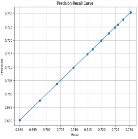
\includegraphics[width=0.5\linewidth]{converted_images/pr-curve.pdf}
    \textbf{Image 15:} Precision-recall curve.
\end{figure}

% author work
\hspace*{1.00cm} This result emphasizes the need for data analysis and potential improvements in the problematic classes, rather than focusing solely on changes to the model's hyperparameters. Additionally, if the "problematic" classes did not exist, Precision and Recall would remain at a constant \texttt{100\%}, resulting in a flat curve.

\hspace*{1.00cm}By examining the graph, it is evident that in each precision-recall pair, both members are equal, which is a clear indicator of the existence of problematic classes.
Evaluation of the best point of grid search indeed confirms existance of problematic classes.

\subsubsection*{Class results and handling of problematic classes}

% authot work
\hspace*{1.00cm}During the grid search process, the best metrics were achieved at a certain configuration.
Detailed class evaluation for the best grid search point with 50 classes yielded the following results:
(1, 3, 0.82, 0.7305, 0.7305, 0.6770, 2702, 991, 46577, 991) — indicating 991 misclassified images in total.
A closer inspection of these results reveals that some classes perform significantly worse than others, which contributes to the overall misclassification rate.


\begin{figure}[H] \centering 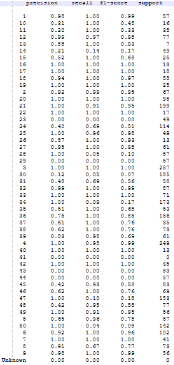
\includegraphics[width=0.4\linewidth]{converted_images/class_metrics (1).pdf} \textbf{Image 16:} Overview of metrics for each class. \end{figure}

% author work
\hspace*{1.00cm}The evaluation shows that some classes achieve excellent results, while others are significantly weaker, thus affecting the overall system performance. Specifically, the table shows the distribution of classes into three performance groups (\texttt{0-49\%}, \texttt{50-74\%}, \texttt{75-100\%}).

\begin{figure}[H]
    \centering
    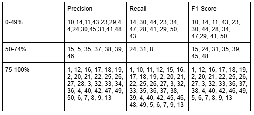
\includegraphics[width=0.7\linewidth]{converted_images/tabelica.pdf}
    \textbf{Image 17:} Performance distribution table.
\end{figure}

\begin{figure}[H]
    \centering
    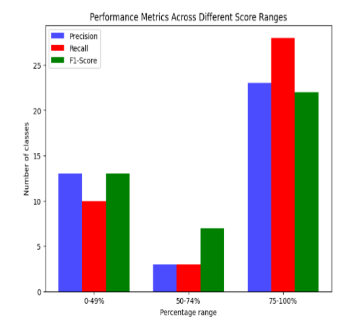
\includegraphics[width=0.7\linewidth]{converted_images/performance_distribution_graph.pdf}
    \textbf{Image 18:} Range-based metrics distribution.
\end{figure}

%author work
\hspace*{1.00cm}By identifying problematic classes that are quite difficult to classify even by eye due to their low quality, we came up with the idea of evaluating the model without these classes. By removing 17 extremely low-quality classes, the best evaluation combination of parameters for the previous dataset was tested, and the following results were achieved:

- Accuracy: 0.8786
- Recall: 0.8786
- F1 Score: 0.8628
- TP: 2295, FP: 317, TN: 9827, FN: 317

\begin{figure}[H]
    \centering
    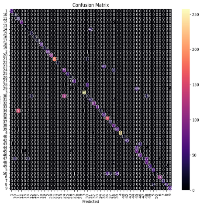
\includegraphics[width=0.70\linewidth]{converted_images/problematic_conf_mat.pdf}
    \textbf{Image 19:} Confusion matrix with problematic classes.
\end{figure}

% ref na neki članak o conf mat

\hspace*{1.00cm}A more detailed analysis of the confusion matrix \cite{geeksforgeeks_confusion_matrix} reveals that there are certain problematic classes that constantly mix with each other. Specifically, these are: 11-34, 39-50, 36-50, 29-49, 48-47, 35-23, 28-30. If we remove some of them, the metrics automatically improve, although not perfectly. It is evident that now the mixes are 36-50, 39-50, 47-6, 34-13, 34-3. Therefore, theoretically, the system could be brought to 
\texttt{100\%} performance through iterative evaluation and elimination of the classes that mix, but this would not be a realistic evaluation. However, removing classes that are simply bad has a significant positive impact on the system.

\begin{figure}[H]
    \centering
    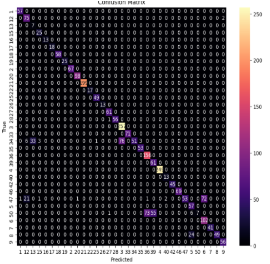
\includegraphics[width=0.70\linewidth]{converted_images/dezinficirani_matrix.pdf}
    \textbf{Image 20:} Confusion matrix without problematic classes.
\end{figure}

% author work
\hspace*{1.00cm}By removing problematic classes from the dataset, there is much less confusion during classification, and the system's performance improves, which is yet another indicator that most of the errors did not arise from the system's implementation, but from classes whose training and validation images have certain flaws that prevent their correct classification. Of course, metrics such as the ROC curve (compressed to the top left) or the P-R curve (diagonal) will still look similar due to the nature of multi-class classification and the large number of true negatives, i.e., the equality of false positives and false negatives.
Next, there are a few examples of train-val pairs:
\begin{figure}[H]
    \centering
    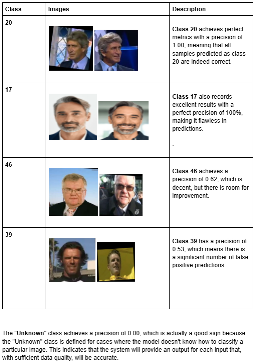
\includegraphics[width=0.7\linewidth]{converted_images/pairs.pdf}
    \textbf{Image 21:} Few class examples.
\end{figure}
\newpage

\subsection*{ROC curve}
\hspace*{1.00cm}
\begin{figure}[H]
    \centering
    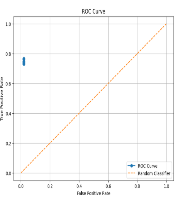
\includegraphics[width=0.7\linewidth]{converted_images/ROC (1).pdf}
    \textbf{Image 22:} Global ROC curve.
\end{figure}

% neki ref na roc curve
\hspace*{1.00cm}The ROC curve \cite{hoo2017roc} in our case does not provide useful information due to the large imbalance between true negative (TN) and true positive (TP) values. Since the classification involves multiple classes, each positive prediction automatically generates negative predictions for all other classes, resulting in a very low False Positive Rate (FPR) and minimal change in the True Positive Rate (TPR). As a result, the ROC curve is compressed into the top left corner of the graph, where it remains almost stationary. Additionally, the false positive and false negative values are always the same because they are interconnected (incorrectly labeling a sample as belonging to the wrong class automatically leads to incorrectly labeling it as not belonging to the correct class).

% author work
\hspace*{1.00cm}Although it does not show progressive changes in TPR, the positioning of the curve in top left corner confirms that the model correctly recognizes positive cases with few false positives. The imbalance arises because for each image, the model must determine 49 times that it does not belong to a class, while it only determines once that it belongs to a specific class.

\subsubsection*{Time-based scalability test}
% neki članak o scalability testovima
 \hspace*{1.00cm}In testing the system's performance, the effect of increasing the number of classes on the loading time was observed, with a specific focus on the phases of converting images into embeddings and loading them into FAISS. \cite{scepanski2024ai}As expected, the loading time did not grow proportionally with the number of classes. Instead of a linear relationship, the system showed disproportionate growth in time (the increase in the number of classes was greater than the increase in execution time), indicating optimized loading processes and scalability. This result suggests that the system can efficiently handle larger numbers of classes without a significant increase in loading time. Expected increase would follow the given formula:
\begin{equation}
\text{Total loading time} = \text{Number of classes} \times \text{Loading time per class}
\end{equation}

\hspace*{1.00cm}
\begin{figure}[H]
    \centering
    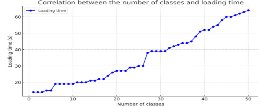
\includegraphics[width=0.7\linewidth]{converted_images/time_scalability.pdf}
    \textbf{Image 23:} Time-based scalability test.
\end{figure}

\hspace*{1.00cm}However, the increase was noticeably smaller. For loading the system with 1 class, it took 14 seconds, while for loading the system with 50 classes, it took 64 seconds. Therefore, with an increase in the number of classes by \texttt{4900\%}, the loading time increased by \texttt{357.14\%}.

\subsubsection*{Metrics-based scalability test}
 \hspace*{1.00cm}The graph shows how the model's performance depends on the number of classes, with Precision, Recall, and F1-score initially remaining at a high level, and a significant drop occurring only after approximately 30 classes. However, the decline in performance is not necessarily only related to the increase in the number of classes, but also to the quality and diversity of the images in the dataset. It is important to note that Precision and Recall consistently align, indicating a balance between the model's accuracy and completeness of recognition. Although all three metrics decrease with the increase in the number of classes, data quality plays a crucial role in maintaining good results. With a well-prepared dataset, the model can maintain high performance even with a larger number of classes. Moreover, by adding high-quality classes, it is possible to improve the metrics, suggesting that the structure, quality, and informativeness of the data has a greater impact on system performance than the number of classes alone.

\begin{figure}[H]
    \centering
    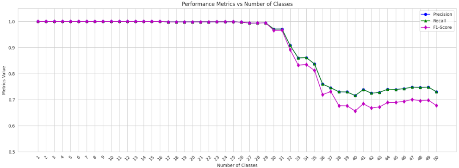
\includegraphics[width=0.7\linewidth]{converted_images/all_metrics_scalability.pdf}
    \textbf{Image 24:} Performance-based scalability test.
\end{figure}
\begin{figure}[H]
    \centering
    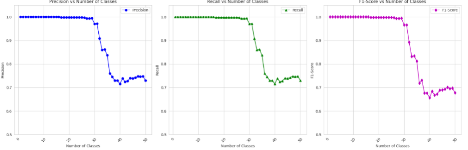
\includegraphics[width=0.7\linewidth]{converted_images/separated_metrics.pdf}
    \textbf{Image 25:} Separeted plots.
\end{figure}

\subsubsection*{Comparison with similar solutions}
\begin{figure}[H]
    \centering
    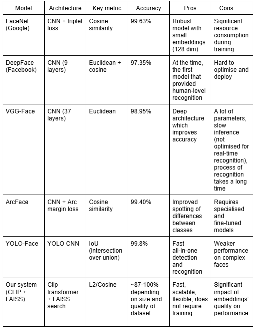
\includegraphics[width=0.7\linewidth]{converted_images/compared (1).pdf}
    \textbf{Image 26:} Table overview.
\end{figure}
% na ovo "train in traditional sense" stavit ref na neki overview modela koje triba trainat
\hspace*{1.00cm}Compared to similar solutions,\cite{thinkingneuron2020facerecognition} our system has certain advantages. Firstly, it does not need to be trained in the traditional sense; new classes/new faces can be added very quickly and easily. Furthermore, the system is extremely easy to implement in applications that involve various forms of face detection without requiring excessive modification, as the operating principle remains unchanged. Additionally, due to CLIP's strong capabilities in extracting embeddings, with a quality dataset, it enables successful recognition of an exceptionally large number of different faces, especially if the conditions for capturing reference images to be added to the system are predefined. It is particularly interesting that successful recognition does not require the live detection input to capture the entire face. The system is not limited by head coverings, masks, etc. If a face is still sufficiently recognizable even with such coverings, the system will classify it correctly. The key is that the system successfully identifies specific parts of the face that contribute most to distinguishing an individual from others.
\begin{figure}[H]
    \centering
    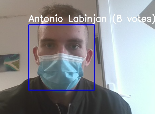
\includegraphics[width=0.5\linewidth]{converted_images/me.pdf}
    \textbf{Image 27:} Example for live detection for covered face.
\end{figure}
\subsection*{Real-life applications}
% ovo je full autorski work
\hspace*{1.00cm}The described system can be implemented for real-time face detection and recognition using a computer camera by passing camera frames as input, creating a bounding box around each detected person, extracting embeddings, and passing them into the described system. The predicted most likely class (with the most votes) is returned as the function's output and added as a label on the box. Additionally, the system can handle multiple known faces simultaneously in the same frame, which adds an extra dimension to the system and enables more advanced recognition in complex situations. It is also important to note that faces can be classified in challenging conditions such as low-light environments. This implementation provides numerous possibilities, such as creating systems for student attendance tracking, payroll calculation based on hours worked, security systems, various interactive interfaces, and more. The system's latency is under 50 ms, and it can process around 200 frames per second, which is an indicator of fairly good performance.
\begin{figure}[H]
    \centering
    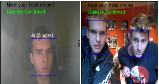
\includegraphics[width=0.8\linewidth]{converted_images/live_2.pdf}
    \textbf{Image 28:} Example for live detection for multiple faces.
\end{figure}
\subsection*{Limitations and conclusions}
\hspace*{1.00cm}Face recognition analysis has shown that image quality and background significantly impact the model's accuracy. When backgrounds are too varied, embeddings become less precise, making it harder to correctly recognize individuals. Additional challenges arise from text, objects in the frame, and large lighting changes, as these introduce variations that are not related to the identity of the person but to the environment.

\hspace*{1.00cm}This problem is particularly evident when the system works with a large number of different faces — while the model achieves high accuracy under controlled conditions, its performance may decline if the data varies in lighting, capture angle, or image quality. Factors such as blurring, low resolution, and contrast can further reduce the reliability of recognition.
To improve results, it would be beneficial to standardize the conditions for capturing reference images or apply methods that ensure greater consistency in input data. For example, in a system for automated student recognition at a university, it would be advisable for all reference images to be captured under the same conditions and with a uniform background, which would neutralize recognition errors.

\hspace*{1.00cm}In conclusion, the results show that the system does not have issues with face recognition, but its accuracy is most affected by external factors that can degrade the quality of the embeddings.

% tu neki ref na pregled tradicionalnih metoda koje koriste CNN
\hspace*{1.00cm}Unlike traditional methods that rely on deep convolutional networks
 specialized for faces, our system uses multimodal embeddings, offering greater flexibility and greater application in various recognition scenarios. Furthermore, the integration of FAISS indexing allows for extremely fast searches, significantly improving the efficiency and responsiveness of the model in real-time. Thus, this work contributes to the field of computer vision, presenting a new methodology that combines the power of transformer embeddings and optimized vector search, opening opportunities for future research and improvements in fast and scalable face recognition.

%\nocite{*} % neka stane ovako za sad, pa ću povezat s konkretnima djelovima lipje pole
% nema baš puno referenci, pošto je većinom "original" work, ali pogledat ću dali ima još ča pametno

% vidit ako moren naj još kakove pametne reference. I povezat svaku referencu na smisleno misto u tekst
\bibliographystyle{plain}  % ili ieee, alpha, apa... ovisi o pravilima
\bibliography{sources}      % bez .bib ekstenzije
\end{document}

% ref na pregled konkurencije odnosno onu tabelu
% dosljedno citirat sva ponavljanja pojmova